\chapter{Introduction}

The automated droplet flow system was set up to perform the polymerisation of P3HT via a Grignard Metathesis method outlined by Loewe et. al.[REF]. P3HT was selected as the synthetic product for the system as it is a well-researched material, relevant in current device fabrication technologies, and has a well-understood mechanism. In this introduction and literature review, first the synthesis of poly(thiophene)s will be discussed to provide an understanding of the mechanism behind the synthesis investigated in this project. Following this, the operation of a flow reactor and gel-permeation chromatography will be explained. Finally, an introduction to self-optimisation will be presented, to show the relevance of optimisation in chemistry, why the developments to the flow reactor outlined in the project were necessary.

\section{Poly(thiophene) }
Poly(thiophene)s (PTs) are a widely-studied class of organic polymer that exhibit semiconducting properties due to their delocalised -system. The chains are formed from repeating thiophene units, i.e. sulphur –substituted pentene aromatic rings. Figure 1 shows the structure of thiophene, poly(thiophene) and the substituted polymer P3HT used in this project.

\begin{figure}[h]
\centering
\includegraphics[scale=0.6]{Thiophenes}
\caption{\textbf{Polythiophene Structure:} From left to right is shown the chemical structure of thiophene, poly(thiophene) and poly(3-hexylthiophene)
}
\centering
\end{figure}

Organic semiconductors have been used to fabricate a wide range of electronic devices including solar cells[REF], LEDs[REF] and transistors[REF]. Over the years, the development of organic semiconductors has included more complex chemistries such as block copolymers[REF] and hybrid organic-inorganic blends. However, simpler poly(thiophene) chemistries are still used in current technology.

\subsection{Synthesis of Poly(thiophene)}

The use of organic semiconductors to fabricate electronic devices has been widely popular since the first organic device in X [REF], with applications to solar cells [REF], LEDs [REF] and transistors [REF]. A variety of substituted polythiophenes have been applied to organic electronics, with papers drawing comparisons of different thiophene chemistries[REFs]. A polymer that displays attractive physical, chemical and electronic properties is poly-3-hexylthiophene, or P3HT[REF], which was the focus of the work described in this report. 

\subsection{Synthesis of Poly(thiophene)}

Unsubstitued poly(thiophene) (PT) exhibits low solubility and is poorly suited to solution processing. The earliest synthesis of poly(thiophene) investigated by Yamamoto et. al. and Lin et. al. describes the relative insolubility of higher-weight PT in organic solvents. For the application of poly(thiophene) to organic electronics, the semiconducting material needs to be amenable to thin-film processing[REF]. By adding alkyl groups to the polymer, it is possible to increase the solubility of the polymer in common solvents such as THF, allowing for solution processing.

C. Arbizzani et. al. published a comparison of the poly(alkylthiophenes) (PATs) poly(3-methyl-hexylthiophene) (P3MT) and P3HT. In the paper, he discussed the “increasing attention” toward longer chain PATs as a result of their better solution processability. A multitude of papers in the past have documented the effect of balancing crystallinity and conductivity with solubility for rigid semiconducting polymers, such as the review of polyaniline chemistry by A. G. MacDiarmid et. al.[ref] and the structural study of doped polymers by R. H. Baughman et. al.[REF]. Whilst larger alkyl chains improve solution processability, the conductivity of the material decreases. Poly(alkylthiophene)s, particularly P3HT display a good balance of conductivity and solution processability[REF].


\subsection{Synthesis of Poly(alkylthiophene)}

A wide variety of methods have been reported for synthesising poly(alkylthiophene)s (PATs). Osawa et. al. reported an electrochemical route, in which an ultrasonic field was placed over the reaction to afford a PAT film, with the ultrasonic radiation preventing the formation of macromolecules as the film was grown. An oxidative polymerisation utilising a FeCl3 catalyst was later reported by Sugimoto et. al., and shown by Leclerc et. al. to yield a material with a higher level of crystallinity than electrochemical methods, an important morphology change that results in increased conductivity. A third method, first published by Jen et. al., employed a nickel complex to catalyse the polymerisation of a thiophenyl Grignard reagent. This method, known as the Kumada cross-coupling method, can be seen in Figure 2. 

\begin{figure}[h]
\centering
\includegraphics[scale=0.6]{Couplings}
\caption{\textbf{The Kumada Cross-Coupling of Poly(thiophene):} A 2,4 di-substituted thiophene monomer is polymerised by the nickel catalyst nickel(II)(1,3-bis(diphenylphosphino)propane)chloride. Three coupling orientations, 2.2 - 2.4 can be formed.}
\centering
\end{figure}

The Kumada cross-coupling method can produce PATs of higher molecular weight than the FeCl3 or electrochemical methods, but due to the lack of selectivity of the catalyst, a mixture of head-to-head (H-H), head-to-tail (H-T) and tail-to-tail (T-T) couplings occur (see Fig 2.) The different couplings of each additional monomer, shown in Figure X, resulting in a regiorandom polymer.

\subsection{Synthesis of Regioregular Poly(alkylthiophene)}

H-H couplings introduce unfavourable interactions between the two alkyl chains because of steric hindrance. The result is a twisted polymer backbone, both breaking conjugation and reducing the crystallinity of the polymer. This therefore affects the conductivity of the PAT thin film, with a greater number of H-H couplings present in the polymer chain resulting in a lower conductivity. R. Maur et. al. published a report that demonstrates the effect of regioregularity in P3HT on solar cell efficiency indicating the importance of highly regioregular materials. 
Following on from the demand for regioregular PAT synthesis, a variety of synthetic methods were published, such as A. Iraqi et. al. for instance outlined a palladium catalysed pathway and S. Guillerez et. al. who reported a Suzuki coupling process. However, the two methods that provided the highest regioregularity were the Grignard metathesis with a nickel catalyst pioneered by McCullough et. al., and the organozinc metathesis published by Rieke et. al.

\subsection{McCullough Synthesis via Kumada Coupling Method}

The synthesis outlined by McCullough et. al. can be seen in Figure X. A 5-bromo thiophene is reacted with the Grignard reagent MgBr2.OEt2 to generate the active monomer species. By performing the reaction at -78 C, the kinetic product 3.2 forms more readily than the monomer 3.3 in a 99:1 ratio, important in the formation of solely (H-T) couplings. The nickel complex Ni(dppp)Cl2 (dppp = diphenylphosphinopropane) is then used to polymerise the Grignard monomer via a cross-couple mechanism. The PATs synthesised by this method displayed a regioregularity (RR) of 98 \%.

\begin{figure}[h]
\centering
\includegraphics[scale=0.5]{McCullough}
\caption{\textbf{The McCullough Method of Poly(alkylthiophene) Synthesis:} A 4-bromo-3-alkylthiophene is treated with a Grignard reagent to form two isomers of the active Grignard species. The monomers are then polymerised with the nickel(II)(1,3-bis(diphenylphosphino)propane)chloride catalyst to form the poly(alkylthiophene).}
\centering
\end{figure}


\subsection{Rieke Synthesis via Negishi Cross-Coupling Method}

The reaction scheme for the synthesis reported by Rieke et. al. can be seen in Figure 4. A dibromothiophene is reacted with “Rieke Zinc”, finely powdered zinc to generate two organozinc species 4.2 and 4.3 in a 9:1 ratio. The polymerisation is then catalysed by Ni(dppe)Cl2 (dppe = 1,2-bis(diphenylphospino)ethane) to afford PATs with a RR \textgreater 97 \%.

\begin{figure}[h]
\centering
\includegraphics[scale=0.5]{Rieke}
\caption{\textbf{The Rieke Method of Poly(alkylthiophene) Synthesis:} A 2,4-dibromo-3-alkylthiophene is reacted with a fine zinc powder to form two isomers of the active organozinc species. The monomers are then polymerised with the catalyst nickel(II)(1,3-bis(diphenylphosphino)ethaane)chloride to form the poly(alkylthiophene).}
\centering
\end{figure}

\subsection{GRIM Synthesis}

The next development in PAT synthesis was outlined in a publication by Loewe et. al., which was termed the Grignard metathesis polymerisation method, or “GRIM” polymerisation. A summary of the reaction can be seen in Figure 5.  The reaction chemistry, whilst similar to the chemistries in schemes 3 and 4, further improved the regioregularity whilst also eliminating the need for low temperatures. The generation of the two Grignard species 5.2 and 5.3 afforded a ratio of 85:15 respectively, notably lower than previous methods. This low ratio arose due to the reflux conditions in which the Grignard metathesis was performed causing metal-halogen exchanges to occur. Although the increased fraction of the unwanted component might have been expected to result in a lower final regioregularity, upon polymerisation the product PAT displayed a RR \textgreater 99\% and a low polydispersity (PD), in the range of 1.2 – 1.4.

\begin{figure}[h]
\centering
\includegraphics[scale=0.5]{GRIM}
\caption{\textbf{The GRIM Polymerisation of Poly(alkylthiophene) Synthesis:} A 2,4-dibromo-3-alkylthiophene is reacted under reflux with a Grignard reagent to form two isomers of the active Grignard monomer. The monomers are then polymerised with the catalyst nickel(II)(1,3-bis(diphenylphosphino)ethaane)chloride to form the poly(alkylthiophene) of high regioregularity and low PD.}
\centering
\end{figure}

Upon further investigation into the reaction by Loewe et. al., the chemical structure of the nickel catalyst was shown to have a large effect on the regioregularity. The highest RR was obtained when catalysts with small metal centres and bulky organic ligands were used, such as 1,3-bis(diphenylphosphino)propane (dppp) and 1,2-bis(diphenylphosphino)ethane (dppe). Whilst the bulkiness of the catalyst supports the theory that steric hindrance causes the high regioregularity by preventing the formation of H-H couplings, this does not account for the lack of T-T couplings, as T-T displays the least steric hindrance. In 2005, Iovu et. al. proposed a living polymerisation mechanism for the growth, as outlined in Figure 6.
The GRIM Polymerisation of Poly(alkylthiophene) Synthesis: A 2,4-dibromo-3-alkylthiophene is reacted under reflux with a Grignard reagent to form two isomers of the active Grignard monomer. The monomers are then polymerised with the catalyst nickel(II)(1,3-bis(diphenylphosphino)ethaane)chloride to form the poly(alkylthiophene) of high regioregularity and low PD.

\begin{figure}[h]
\centering
\includegraphics[scale=0.5]{Catalyst_Generation}
\caption{\textbf{Mechanism of the GRIM Polymerisation Method: Part A:} Two equivalents of the active Grignard thiophene species (6.2) undergo substitution with the chloride ligands of nickel(II)(dppp)chloride complex (6.1). The complex the undergoes reductive elimintation to form the active catalyst (6.6) and a T-T coupled dithiophene molecule (6.5). The catalyst then undergoes oxidative addition at one of the C-Br bonds of the dithiophene. \textbf{Mechanism of the GRIM Polymerisation Method: Part B:} The catalyst cycle begins with the substitution of an additional monomer (6.8) to the catalyst centre to form the species (6.9). The catalyst then undergoes reductive elimination, increasing the polymer chain length and reforming the active catalyst. The active catalyst then undergoes oxidative addition with the C-Br bond at the polymer end to complete the cycle.}
\centering
\includegraphics[scale=0.5]{Catalyst_Cycle}
\centering
\end{figure}

Upon formation of the activated Ni(0) species 6.6, the bithiophene molecule 6.5 and nickel species inserts into the carbon-bromine bond via oxidative addition. The species then undergoes transmetallation followed by insertion of a new monomer into the chain to form intermediate 6.9. It had previously been assumed that a free Ni(0) complex and a polymer chain were then formed by reductive elimination. However, the data shown in Figure 7A shows both the monomer concentration and weight average against conversion. 

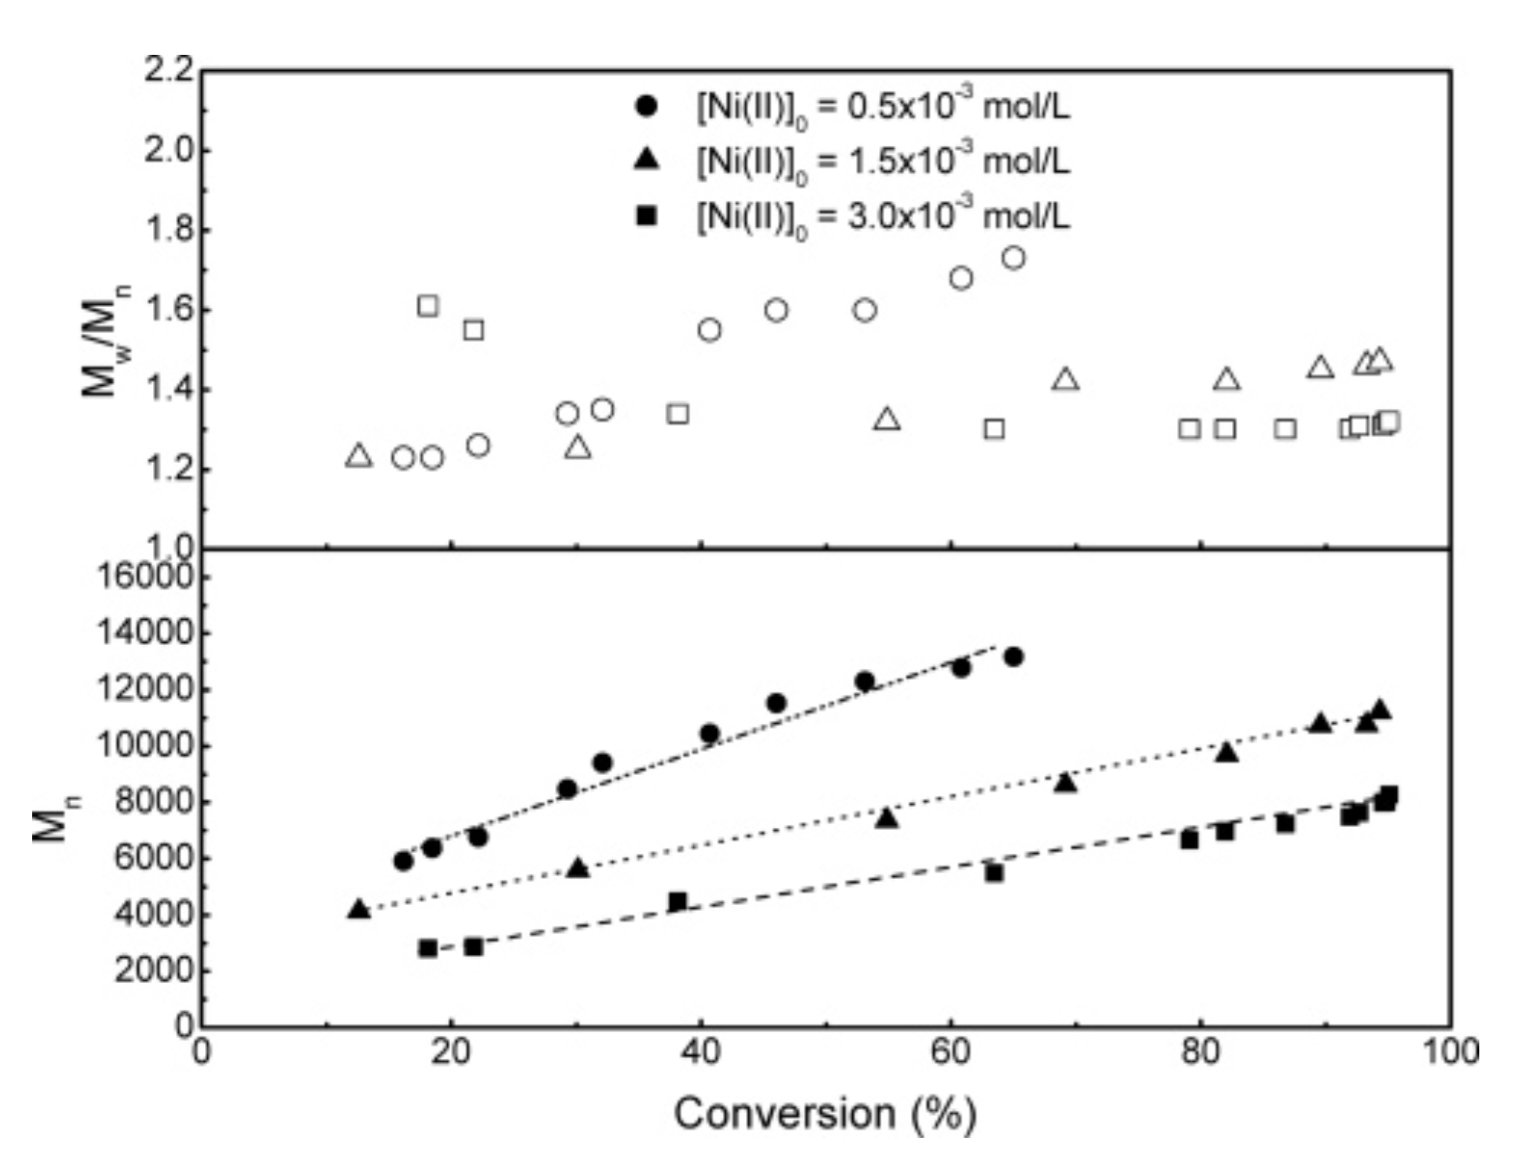
\includegraphics{Quasi_Liv_1}

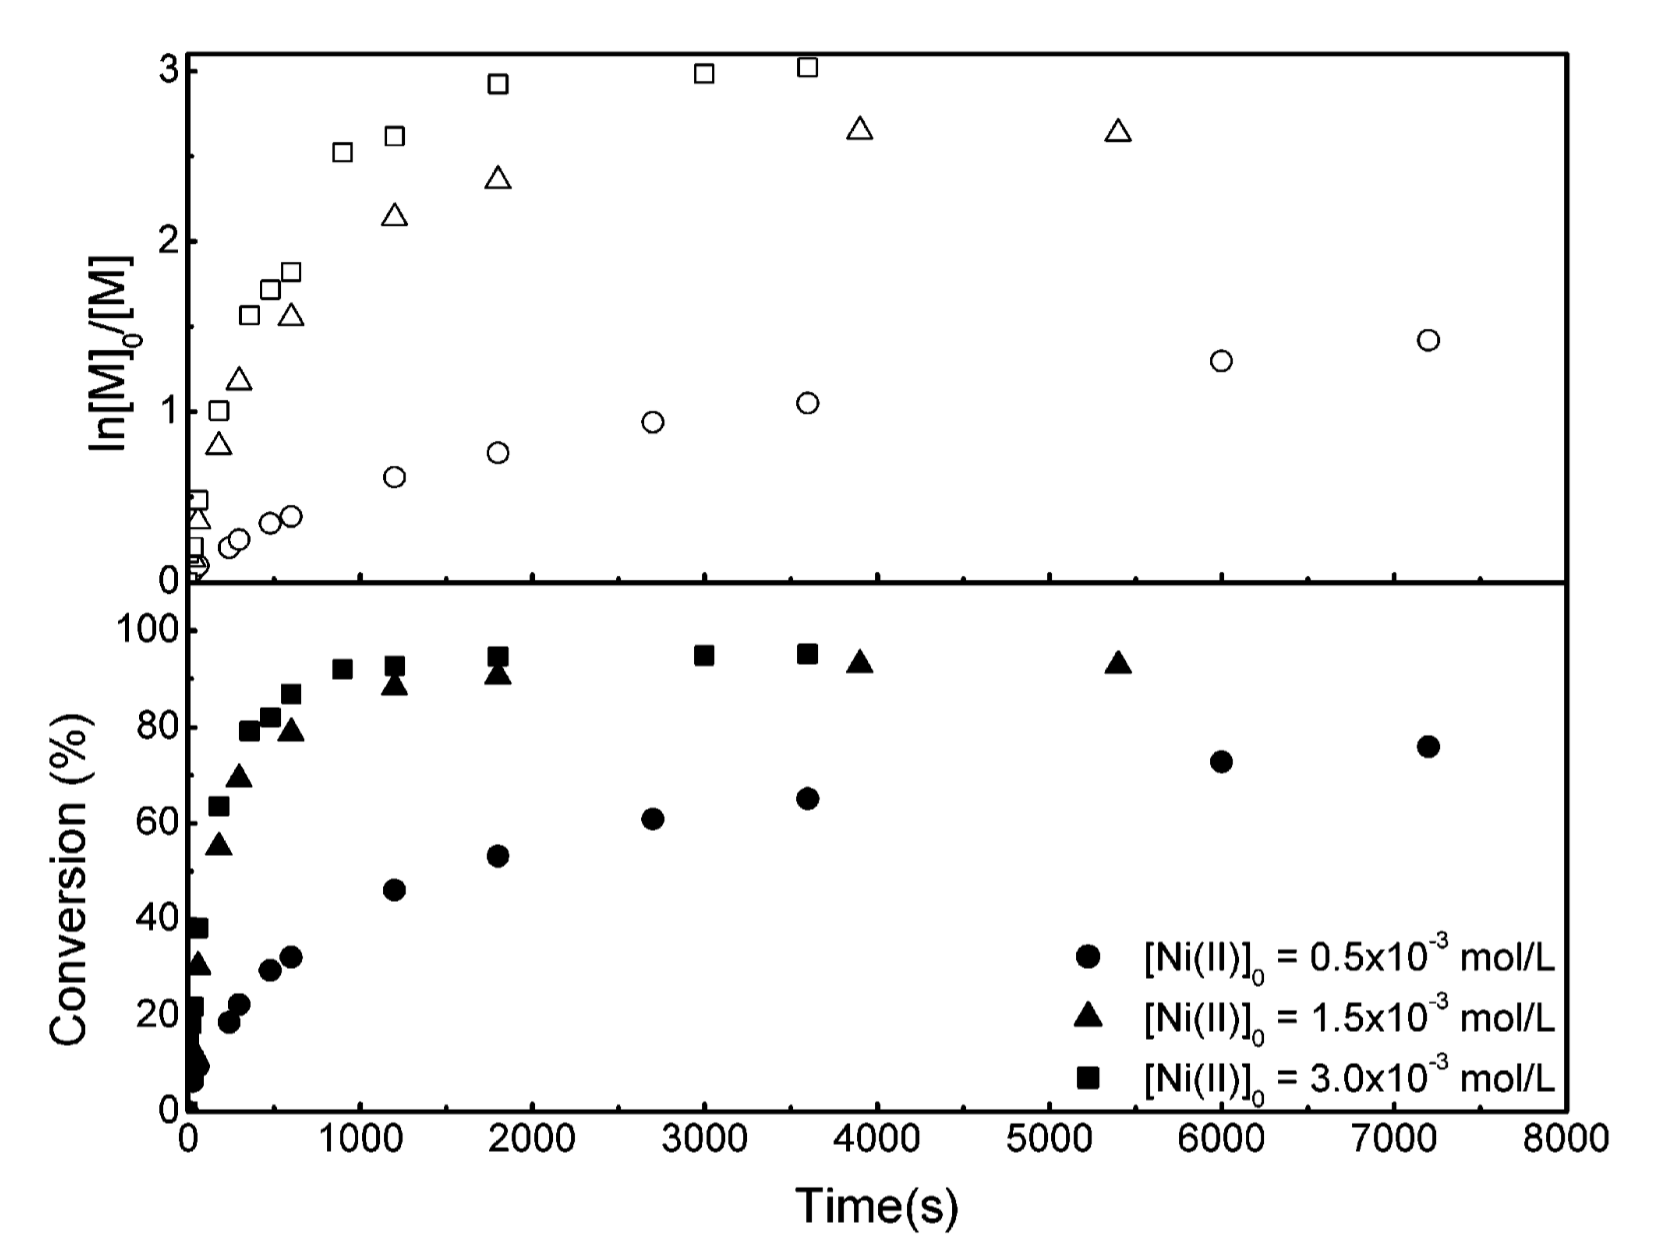
\includegraphics{Quasi_Liv_2}

The data shows increase in reaction rate with increasing catalyst concentration. Furthermore, the linear trend seen in Mn against conversion indicates a living chain growth. However, as seen in Figure 7B, conversion rate and change in monomer concentration decreases at approximately 60 \% conversion. Therefore, the system can be described as quasi-living chain growth. The mechanism is thought to form a structure termed an “associated pair” where the Ni(0) complex is attracted to the eliminated chain as seen in 6.10 and 6.11. The complex then acts as an initiator for the polymerisation at the chain end. In further support of this mechanism, the NMR of polymers synthesised by the GRIM method show a singlet response with an integral of 1, indicative of one T-T coupling present in each polymer chain. This is expected for the mechanism shown in Figure 6 since the initial dimer 6.5 formed consists of a single T-T coupling. 

The high regioselectivity, ability to carry out the synthesis at ambient temperatures affords the reaction to be amenable to translation from a batch reactor to a flow reactor, as demonstrated by Bannock et. al. [REF] in his synthesis of P3HT of low PD (1.2 - 1.7) through a modified version of the GRIM method. 

\section{Flow Chemistry}

Flow chemistry involves the use of continually flowing streams of reactant solutions to perform chemical reactions. This provides an alternative method to the traditional batch method of chemical synthesis, often eliminating issues with the translation of small scale to large scale processes due to flow chemistry providing excellent reagent mixing and heat transfer even at the large scale. 

A paper published by Bannock et. al. highlighted the ease of constructing a flow reactor, and aimed to demonstrate the facile nature of translating a chemical reaction to a flow system for the research environment. The paper highlighted issues that can arise in a flow chemical process. A viscous solution can result in high back pressures in the system that can restrict pumping, whilst gas evolution and solid precipitation can cause blockages and leaks that damage the reactor. However, benefits such as the ease of mixing can greatly improve the quality of a chemical product. Due to the relatively small immediate volumes within a flow reactor, the rate of diffusion of reactants to reactant sites within a solution can be greatly improved on those in a batch process. The mixing of two liquid streams in a flow system can result in two different phenomena, known as laminar flow and droplet flow, shown and described in Figure 8.

\includegraphics{Flow_Mixing}

Of particular interest to the synthesis of polymers with low PD is the phenomena seen in Figure 8B. When two immiscible fluids are mixed together, discreet segments of alternating solutions can be formed, known as droplet flow. The liquid with a higher wetting coefficient to the tubing material used acts as a “carrier fluid” that transports discrete “droplets” of the second liquid. By isolating a chemical reaction within these droplets, each act as a miniature batch reaction. This allows for good control of reactant diffusion and heat flow, and so a uniform reaction environment over a large total volume of reactant solution. Bannock et. al. was the first to report conjugated polymer synthesis by a droplet flow method, and designed a flow reactor that used this droplet-flow method to synthesise P3HT via the GRIM method outlined in section 1. The reactor used an inert polyfluoropolyether (PFPE) called Galden, a viscous liquid containing a uniform dispersion of the nickel catalyst to transport droplets of a thiophene Grignard reagent, as shown in the schematic Figure 9 below. 

\includegraphics{BannockReactor}

The droplet stream then entered a heated oil bath to induce the polymerisation. The resulting P3HT was of high RR (\textgreater 98 \%) and low PD (1.2-1.7), and the Mw could be easily controlled through the temperature and flow parameters of the system, up to a Mw of 92 kDa. Unlike the batch synthesis which encounters isssues with increasing viscosity with the synthesis of higher Mws, the small reaction volumes of the droplet flow system result in short diffusion distances for the monomer reagent to reach the active chain ends. Bannock et. al. then demonstrated the synthesis of copolymers of P3HT and P3HS, a selenium-substituted thiophene. By varying the ratio of the thiophene and selenophene reactant flow rates, copolymers of matching stoichiometry could be synthesised. This showed the ability for ease of polymerisation control through the facile control of reagent flow rates.


\section{Gel Permeation Chromatography}

Size exclusion chromatography (SEC) is an analytical method of determining the molecular weight properties of a polymer through separation based on the molecule size and volumetric properties. One type of SEC, involving the polymer dissolved in an organic solvent passing through a solid porous gel matrix, is also known as gel permeation chromatography (GPC). Figure 9 shows the operation of a GPC column.

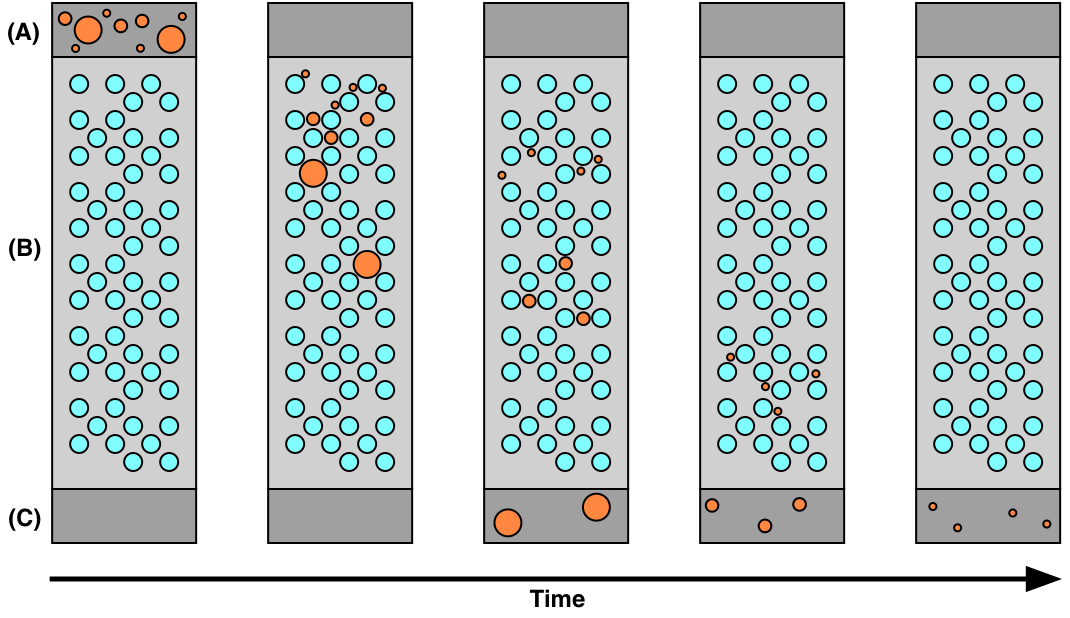
\includegraphics{GPC_Operation}

The column of a GPC is coupled to a detector located at the output. The detector is designed to produce a response based on the material passed through the column. Common detectors probe the sample’s refractive index(REF) or absorption in either the UV(REF) or IR(REF) region. Other detection method, such as light scattering methods(REF) are available.

A typical GPC output can be seen in Figure 10. The axes are plotted with the detector signal against the time that the sample has been present in the column, known as the retention time. The x-axis can also be displayed in the unit ‘retention volume’, which is calculated from the volumetric flow rate of sample injection. The signal obtained increases with increasing polymer concentration at the detector, with the larger polymer eluting through the system faster than the smaller polymer chains. Therefore, a broad signal indicates a large range of polymer chain lengths in the sample, whereas a sharp signal indicates a high degree of uniformity in polymer chain length. This property is quantified in the property polydispersity (Đ). The molecular weight dynamics of semiconducting polymers, such as P3HT, have a large effect on the quality of electronic devices in which they are included(REF), and therefore are important properties to investigate. Whilst different average molecular weights have applications to different electronic devices, most applications require polymers with a low Đ. 

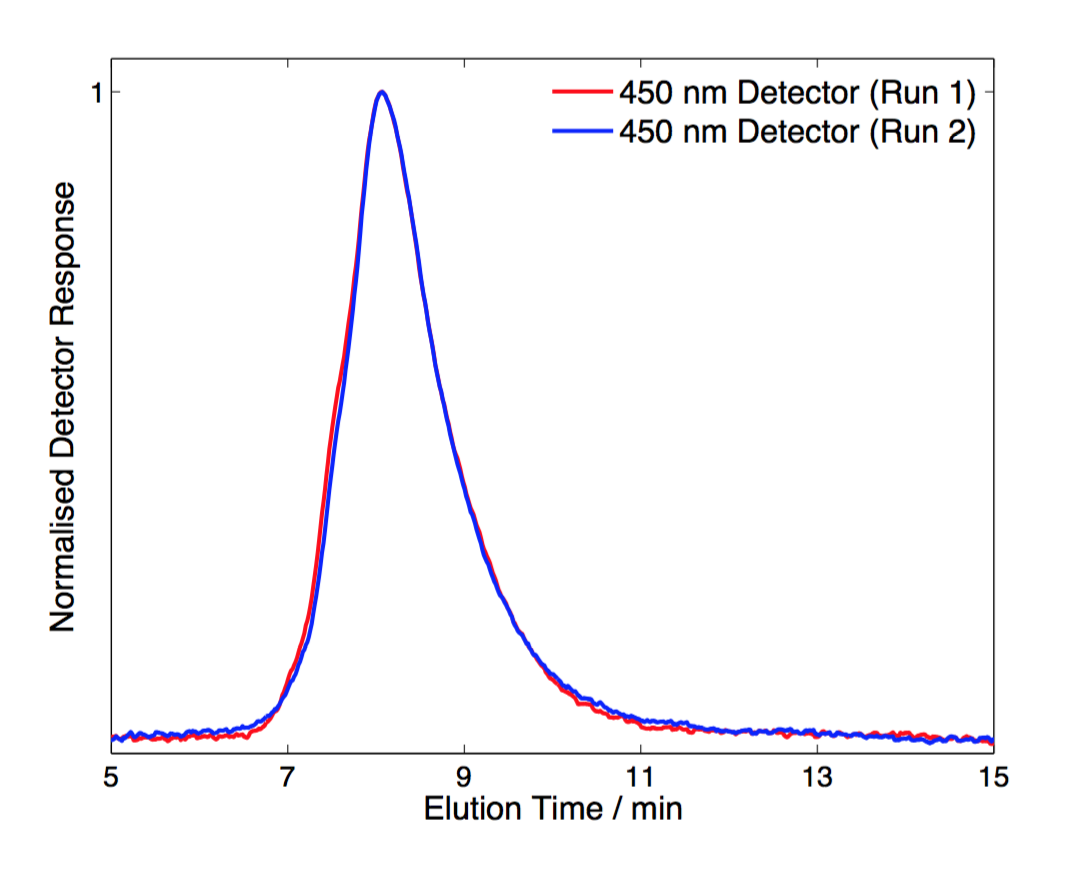
\includegraphics{ExampleGPC}

\subsection{GPC Calibration}

A wide variety of source materials are available for the calibration of GPC instruments. The book “Handbook of Size Exclusion Chromatography” published by C. Wu highlights the variety of calibration methods. The simplest method, used in this project, is known as Direct Standard Calibration (DSC). DSC is an appropriate calibration method for linear samples of low Đ, but it has been shown that more complex polymers, particularly branched dendrimers, require a more sophisticated calibration. Furthermore, samples with large Đ can give an inaccurate reading.
DSC requires a calibration set, which consists of multiple polymer samples of known molecular weight, and a narrow Đ which should be 1.2 or below. Each sample is run through the GPC, providing a value of retention time for the molecular weight in question. A calibration plot can then be constructed of retention time against the log of molecular weight. An example calibration can be seen in Figure 11.

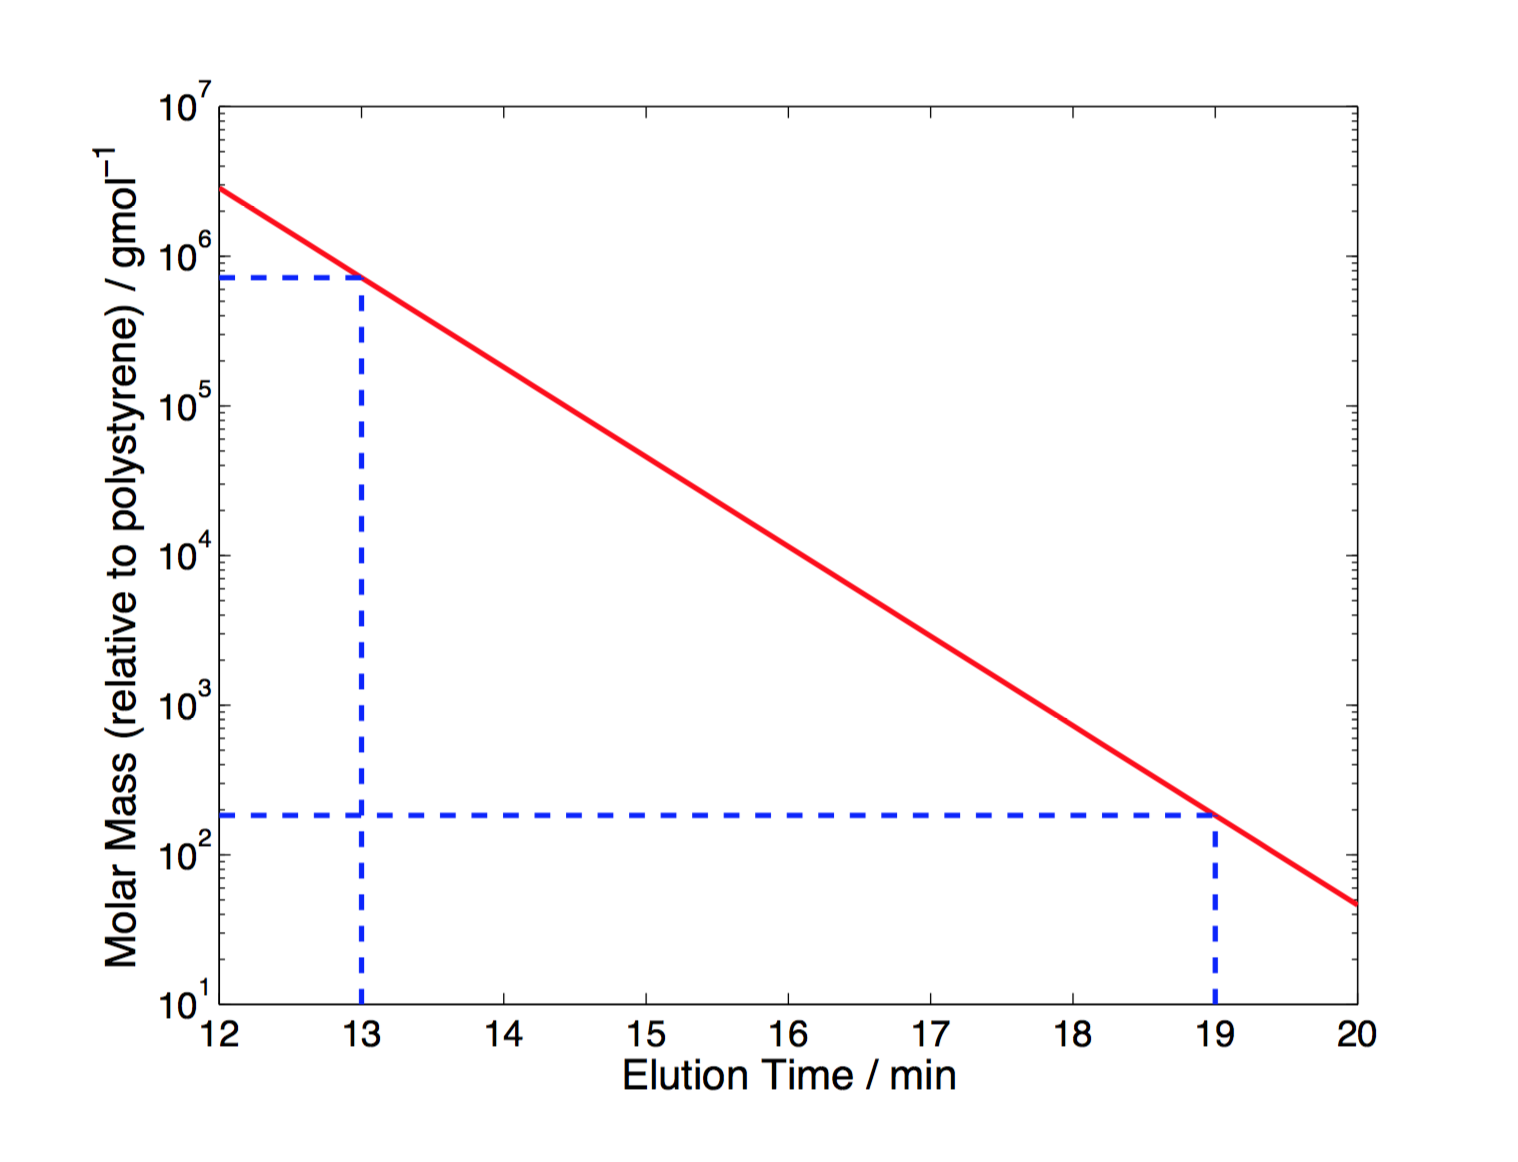
\includegraphics{CalibExample}

The calibration curve becomes the reportable range in which an accurate measurement can be taken. For this reason, a wide calibration set is necessary to create an instrument able to analyse a wide range of samples.

\section{Automation}

The application of automation of chemical reactions and processes provides an ideal solution to the demand for repeated experimentation and consistent and accurate test conditions vital to both research and industry. A study on the effect of laboratory automation in the medical profession over the last 36 published in 2003 by Sarkozi et. al. demonstrates the efficacy of automation. Figure 12 shows a graphical depiction of the volume of tests performed per employee at an institution are shown alongside the cost per test, as well as the number of employees against the gross number of tests performed per year.

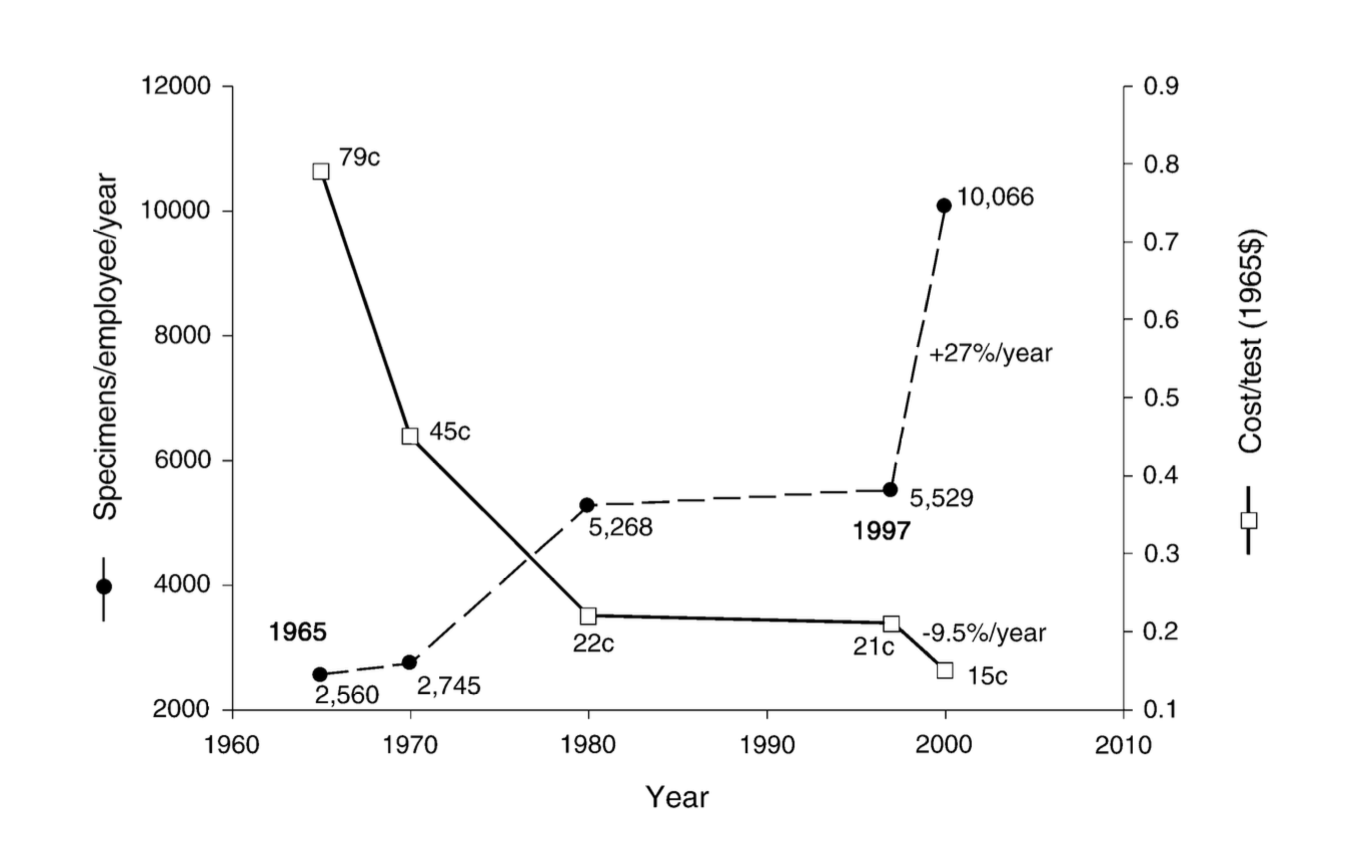
\includegraphics{Auto1}
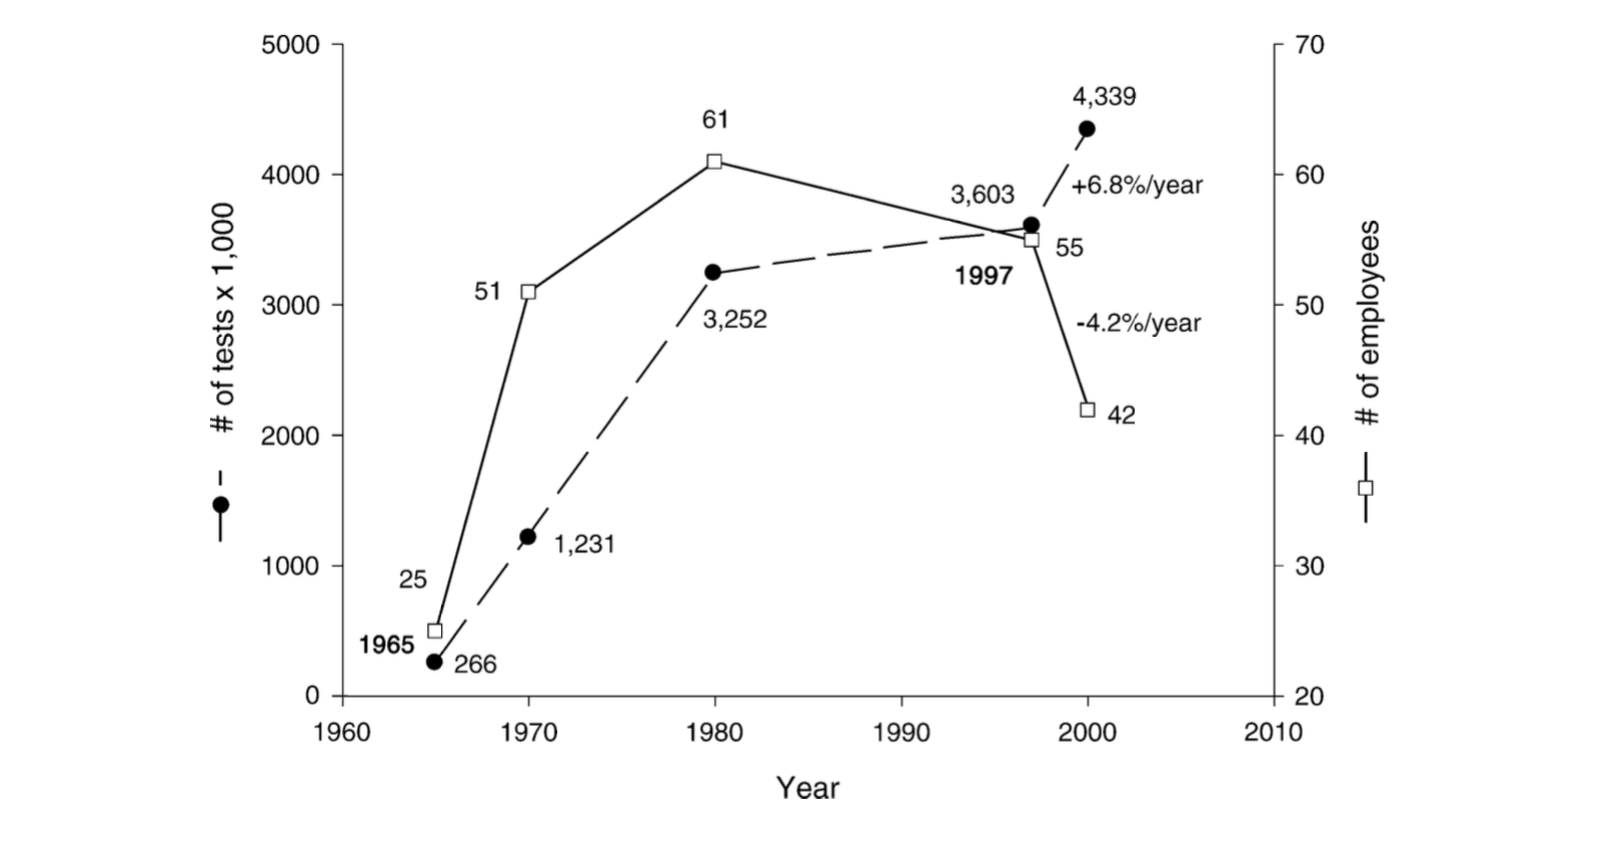
\includegraphics{Auto2}

Notable changes in trends seen in the data could be attributed to the introduction of automated system to the institution. The increase in productivity seen between 1965 and 1980 coincided with the introduction of multi-test analysers that had a much higher sample throughput rate. The installation of a robotic analysis system in 1998 can be attributed to the increase in productivity seen after 1997. Even though there was a reduction in staff numbers by 24 \%, the number of tests performed increased by 6.8 \% a year.
Automated flow chemistry is a recent advancement in flow chemistry technology. A simple diagram for the operation of a self-optimising flow reactor can be found in the review by M. Rasheed et. al., shown in Figure 13. 

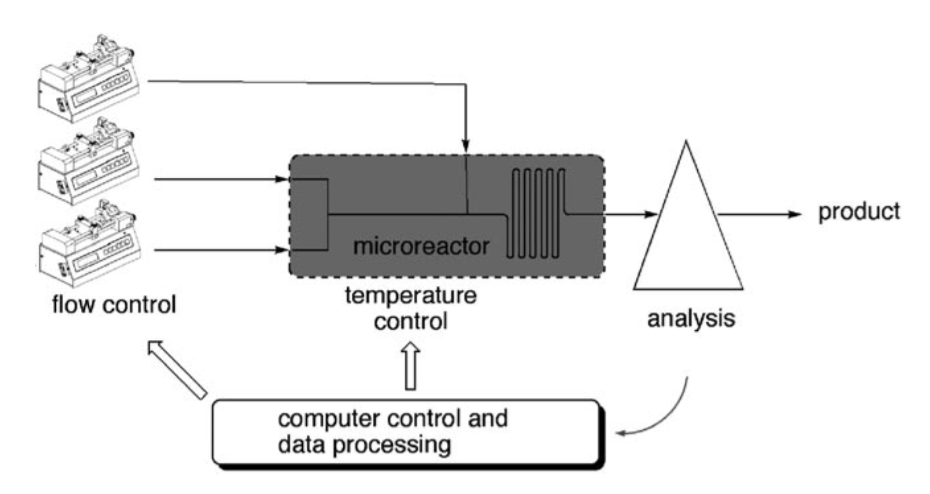
\includegraphics{autoskel}

The ‘hands-off’ approach is appropriately referred to as a black box system. Desired product properties are input to the system, and through a combination of analysis, data processing and automated control of reaction conditions the system can reach the target product through multiple iterations without manual interaction.

This basic operating principle can be tailored to be applicable to a variety of synthetic pathways. If a product can be accurately described from any quantifiable analytical technique in-line, parameters such as reaction temperature, reactant flow rate and stoichiometric flow ratios can be remotely controlled to reach the optimal conditions for the target product property under analysis.

The optimisation of the system is controlled by an optimisation algorithm. The algorithm aims to assign a quality value to the product of a collection of parameters, and from that intelligently suggest new reaction parameters to investigate. The algorithm employed by the John de Mello research group, such as in the publication by Krishnadasaan et. al. investigating inorganic nanoparticles, is known as the SNOBFIT (Stable Noisy Optimisation by Branch and Fit) algorithm. This algorithm, developed by W. Huyer and A. Neumaier, uses response surface methodology (RSM) to intelligently select successive reaction parameters, the theory of which can be found in X. This was used by B.E. Walker et. al. in the synthesis of o-xylenyl buckminsterfullerene adducts via a Diels-Alder cycloaddition, with the analysis following a similar setup to the reactor in this project, consisting of an HPLC pump connected to a silica column, with the output monitored with an LED and photodiode.

